\documentclass[12pt,a4paper]{article}
%\usepackage[UTF8]{ctex}
\usepackage{amsfonts,amsmath,amsthm,amssymb}
\usepackage{mathtools}
\usepackage{sfmath}
\usepackage{hyperref}
\renewcommand{\familydefault}{\sfdefault}
\usepackage{geometry}
\geometry{left=0cm,right=0cm,top=0cm,bottom=0.1cm, footskip=0cm, includefoot=true}
\pagestyle{empty}
\setcounter{secnumdepth}{4}

\usepackage[all]{xy}
\usepackage{color}
\usepackage{tikz}
\usetikzlibrary{arrows.meta}
\usetikzlibrary{calc}

\usepackage{titlesec}
\titleformat{\section}[block]{\huge\bfseries\sffamily}{\thesection}{1em}{}
\titleformat{\subsection}[block]{\huge\bfseries\sffamily}{\thesubsection}{1em}{}
\titleformat{\subsubsection}[block]{\huge\bfseries\sffamily}{\thesubsubsection}{1em}{}
\titleformat{\paragraph}[block]{\huge\bfseries\sffamily}{\theparagraph}{1em}{}
\titlespacing*{\paragraph}{0pt}{1ex}{0.5ex}

\renewenvironment{proof}{{\noindent\it\textbf{Proof}}\quad\it}{\hfill$\square$}

\newtheorem{thm}[equation]{Theorem}
\newtheorem{cor}[equation]{Corollary}
\newtheorem{lem}[equation]{Lemma}
\newtheorem{prop}[equation]{Proposition}
\newtheorem{defn}[equation]{Definition}
\newtheorem{rem}[equation]{Remark}
\newtheorem{conj}[equation]{Conjecture}
\newtheorem{notation}[equation]{Notation}
\newtheorem{definition}[equation]{Definition}
\newtheorem{remark}[equation]{Remark}
\newtheorem{example}[equation]{Example}
\newtheorem{proposition}[equation]{Proposition}

\newcommand{\Z}{\mathbb{Z}}
\newcommand{\Ext}{\operatorname{Ext}}

\newcommand{\AF}{\mathrm{AF}}
\newcommand{\ESS}[1]{\prescript{#1\!}{}{E}}
\newcommand{\ZESS}[1]{\prescript{#1\!}{}{Z}}
\newcommand{\BESS}[1]{\prescript{#1\!}{}{B}}
\newcommand{\SynSS}{\prescript{\mathrm{syn}\!}{}{E}}
\newcommand{\HF}{\mathrm{H}\mathbb{F}_2}
\newcommand{\Sus}{\Sigma}
\newcommand{\iso}{\cong}
\newcommand{\calSyn}{\mathcal{S}\mathrm{yn}}
\newcommand{\calSp}{\mathcal{S}\mathrm{p}}

% Define tikz colors
\definecolor{lightgray}{RGB}{200,200,200}
\definecolor{llgray}{RGB}{235,235,235}

% draw grid in tikz
\newcommand{\tikzgrid}[4]{\foreach \x in {#1,...,#2} {
        \draw[black!20] (\x-0.5, #3-0.5) -- (\x-0.5, #4-0.5);
    }
    \foreach \y in {#3,...,#4} {
        \draw[black!20] (#1-0.5, \y-0.5) -- (#2-0.5, \y-0.5);
    }
}

\newcommand{\drawarrow}{\draw[-{Stealth[length=1.5mm]}, shorten >=(0.08cm)]}

\title{Extensions on a classical $E_r$-page}
\author{}


\begin{document}

\sffamily
\maketitle
\thispagestyle{empty}

\huge

\begin{sloppy}
\clubpenalty=-100
\widowpenalty=-100

\section{Extensions on a classical $E_r$-page} \label{sec:extenpage}

To state the Generalized Leibniz Rule in terms of the classical Adams spectral sequence, we need to define $f$-extensions not only on homotopy groups but \emph{on the $E_r$-page} as well.

\subsection{synthetic lifts}

\begin{notation}
For a map between classical spectra $f: X\to Y$, consider the associated synthetic map from Notation~\ref{not:fhat}
$$\hat f: \Sus^{0,e(f)}\nu X\to \nu Y.$$
For any $2\le r\le \infty$, we denote the following mod $\lambda^{r-1}$ reduction maps by $\hat f_{r-1}$:
$$\hat f_{r-1}: \Sus^{0,e(f)}\nu X/\lambda^{r-1}\to \nu Y/\lambda^{r-1}.$$
\end{notation}

\paragraph{}

The $E_0$-page of the $\hat f_{r-1}$-ESS is isomorphic to
$$\begin{aligned}
    \ESS{\hat f_{r-1}}_0^{s,t,t-k+e(f)}\iso & E_\infty^{s,t,t-k}(\nu X/\lambda^{r-1})\oplus E_\infty^{s,t,t-k+e(f)}(\nu Y/\lambda^{r-1})\\
    \iso & \big(Z_{r-1-k}^{s,t}(X)/B_{1+k}^{s,t}(X)\big)\oplus \big(Z_{r-1-k+e(f)}^{s,t}(Y)/B_{1+k-e(f)}^{s,t}(Y)\big).
\end{aligned}$$

\paragraph{}
A nontrivial $d^{\hat f_{r-1}}_n$ differential can be interpreted as a map from the subgroup
\begin{equation}\label{eq:eae450fe}
  \ZESS{\hat f_{r-1}}_{n-1}^{s,t,t-k}(X) \subset  Z_{r-1-k}^{s,t}(X)/B_{1+k}^{s,t}(X)
\end{equation}
to the quotient group
\begin{equation}\label{eq:334248d2}
    \big(Z_{r-1-k-n+e(f)}^{s+n,t+n}(Y)/B_{1+k+n-e(f)}^{s+n,t+n}(Y) \big)/\BESS{\hat f_{r-1}}_{n-1}^{s+n,t+n,t-k}(Y).
\end{equation}

\paragraph{}
The differential $d^{\hat f_{r-1}}_n$ is trivial for degree reasons when
$$n<\AF(f)\text{ or }n>r-2-k+e(f).$$

\subsection{extension on the $E_r$ page}
\begin{definition}\label{def:6c076a33}
    Let $x\in Z^{s,t}_{r-1}(X)$ and $y\in Z^{s+n,t+n}_{r-1-n+e(f)}(Y)$ for some
    $$e(f)\le n\le r-2+e(f).$$
    We say that there is an $(f,E_r)$-extension from $x$ to $y$, denoted by
    \begin{equation}\label{eq:b98be76a}
    d_{n}^{f,E_r}(x)=y
    \end{equation}
    if there exists a synthetic $\hat f_{r-1}$-extension
    \begin{equation}\label{eq:a020bad3}
        d_{n}^{\hat f_{r-1}}(x)=\lambda^{n-e(f)} y.
    \end{equation}
    where $x$ is viewed as an element of the subgroup (\ref{eq:eae450fe}) with $k=0$, and $\lambda^{n-e(f)} y$ is viewed as an element of the quotient group (\ref{eq:334248d2}) with $k=0$.

   We say that this $(f,E_r)$-extension in (\ref{eq:b98be76a}) is \emph{essential} if the corresponding synthetic $\hat f_{r-1}$-extension in (\ref{eq:a020bad3}) is an essential differential in the $\hat f_{r-1}$-ESS.

    For $r=\infty$, we similar define an $(f,E_\infty)$-extension using the corresponding synthetic $\hat f$-extension.
\end{definition}



\begin{figure}[h]
\scalebox{0.85}{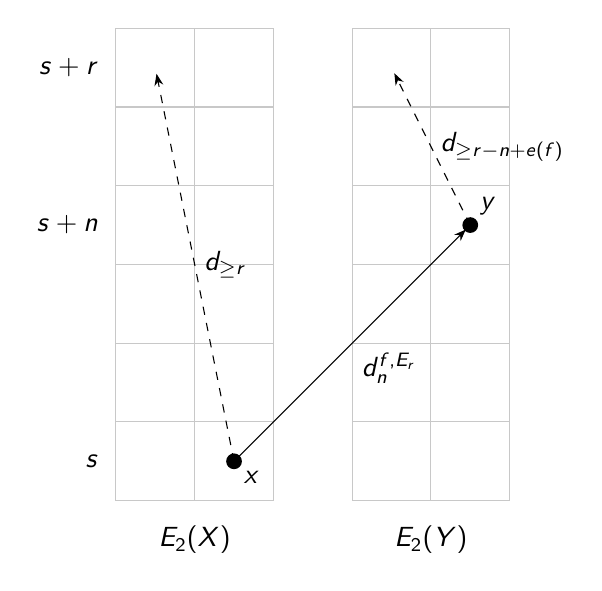
\begin{tikzpicture}
    % Draw grid
    \foreach \x in {0,...,5} {
        \draw[lightgray] (\x-0.5, -0.5) -- (\x-0.5, 5.5);
    }
    \foreach \y in {0,...,6} {
        \draw[lightgray] (-0.5, \y-0.5) -- (1.5, \y-0.5);
        \draw[lightgray] (2.5, \y-0.5) -- (4.5, \y-0.5);
    }

    % Draw bullets
    \coordinate (x) at (1, 0);
    \coordinate (dx) at (0, 5);
    \coordinate (y) at (4, 3);
    \coordinate (dy) at (3, 5);

    \fill (x) circle (0.1) node[below right] {$x$};
    \fill (y) circle (0.1) node[above right] {$y$};

    % Draw differentials
    \draw[dashed, -{Stealth[length=1.5mm]}, shorten >=(0.08cm)] (x) -- (dx) node[midway,right] {$d_{\ge r}$};
    \draw[dashed, -{Stealth[length=1.5mm]}, shorten >=(0.08cm)] (y) -- (dy) node[midway,right] {$d_{\ge r-n+e(f)}$};
    \drawarrow (x) -- (y) node[midway,below right] {$d^{f,E_r}_{n}$};

    \node[anchor=east] (axis1) at (-0.6, 0) {$s$};
    \node[anchor=east] (axis2) at (-0.6, 3) {$s+n$};
    \node[anchor=east] (axis3) at (-0.6, 5) {$s+r$};


    \node (EX) at (.5, -1.0) {$E_2(X)$};
    \node (EY) at (3.5, -1.0) {$E_2(Y)$};
\end{tikzpicture}
\hspace{0.5cm}
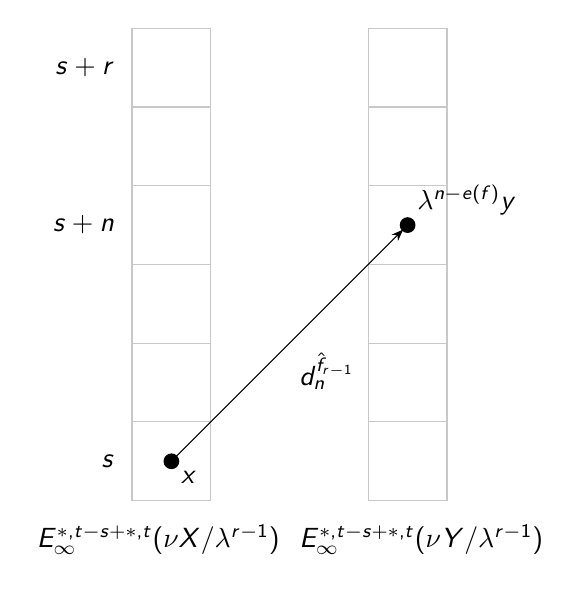
\begin{tikzpicture}
    % Draw grid
    \foreach \x in {0,1,3,4} {
        \draw[lightgray] (\x-0.5, -0.5) -- (\x-0.5, 5.5);
    }
    \foreach \y in {0,...,6} {
        \draw[lightgray] (-0.5, \y-0.5) -- (0.5, \y-0.5);
        \draw[lightgray] (2.5, \y-0.5) -- (3.5, \y-0.5);
    }

    % Draw bullets
    \coordinate (x) at (0, 0);
    \coordinate (y) at (3, 3);

    \fill (x) circle (0.1) node[below right] {$x$};
    \fill (y) circle (0.1) node[above right] {$\lambda^{n-e(f)} y$};

    % Draw differentials
    \drawarrow (x) -- (y) node[midway,below right] {$d^{\hat f_{r-1}}_{n}$};

    \node[anchor=east] at (-0.6, 0) {$s$};
    \node[anchor=east] at (-0.6, 3) {$s+n$};
    \node[anchor=east] at (-0.6, 5) {$s+r$};

    \node[anchor=east] at (1.5, -1.0) {$E_\infty^{*,t-s+*,t}(\nu X/\lambda^{r-1})$};
    \node[anchor=west] at (1.5, -1.0) {$E_\infty^{*,t-s+*,t}(\nu Y/\lambda^{r-1})$};
\end{tikzpicture}
}
\caption{$(f,E_r)$-extension}\label{fig:3d966cc4}
\end{figure}

\begin{definition}\label{def:6c076aw33}
    Let $x\in Z^{s,t}_{r-1}(X)$ and $y\in Z^{s+n,t+n}_{r-1-n+e(f)}(Y)$ for some
    $$e(f)\le n\le r-2+e(f).$$
    We say that there is an $(f,E_r)$-extension of level $l$ from $x$ to $y$, denoted by
    \begin{equation}\label{eq:b98be76aw}
    d_{n}^{f,E_r,l}(x)=y
    \end{equation}
    if there exists a synthetic $\hat f_{r-1}$-extension
    \begin{equation}\label{eq:a020bad3w}
        d_{n}^{\hat f_{r-1}}(\lambda^l x)=\lambda^{n-e(f)+l} y.
    \end{equation}
    where $\lambda^l x$ is viewed as an element of the subgroup (\ref{eq:eae450fe}) with certain $k$, and $\lambda^{n-e(f)} y$ is viewed as an element of the quotient group (\ref{eq:334248d2}).

   We say that this $(f,E_r)$-extension of level $l$ in (\ref{eq:b98be76aw}) is \emph{essential} if the corresponding synthetic $\hat f_{r-1}$-extension in (\ref{eq:a020bad3w}) is an essential differential in the $\hat f_{r-1}$-ESS.

    For $r=\infty$, we similar define an $(f,E_\infty)$-extension of level $l$ using the corresponding synthetic $\hat f$-extension.
\end{definition}

\begin{remark} \label{def:fErextess}
Consider an $(f,E_r)$-extension $d_{n}^{f,E_r}(x)=y$ in (\ref{eq:b98be76a}).
    The element $y$ should be interpreted as a coset with indeterminacy given by $B_{1+n-e(f)}^{s+n,t+n}(Y)$, plus the sum of images of $d^{\hat f_{r-1}}_{<n}$ differentials.   This $(f,E_r)$-extension is \emph{essential} if this coset does not contain 0.
\end{remark}

\subsection{crossings}

\begin{definition}\label{def:41d51149}
    A crossing of the $(f,E_r)$-extension $d_{n}^{f,E_r}(x)=y$ in (\ref{eq:b98be76a}) is defined as an essential $(f, E_{r-a})$-extension from some $x'\in Z_{r-1-a}^{s+a,t+a}(X)$ to
    $$y'\in Z_{r-1-n+b+e(f)}^{s+n-b,t+n-b}(Y)\backslash B_{1+n-b-e(f)}^{s+n-b,t+n-b}(Y)$$
    (where $\backslash$ denotes the difference of sets and it means that $y'$ should survive to the classical Adams $E_{r-n+b+e(f)}$ page while it should not be hit by an Adams differential of length at most $1+n-b-e(f)$) for $0<a \le r-2$ and $0\le b\le n-a-e(f)$. See Figure \ref{fig:66241bf6}.
\end{definition}



\begin{figure}[h]
\scalebox{0.8}{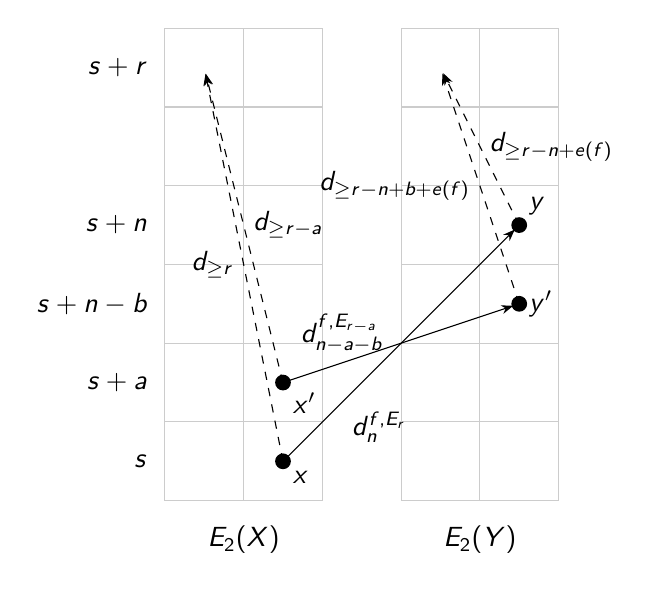
\begin{tikzpicture}
    % Draw grid
    \tikzgrid{0}{2}{0}{6}
    \tikzgrid{3}{5}{0}{6}

    % Draw bullets
    \coordinate (x) at (1, 0);
    \coordinate (x1) at (1, 1);
    \coordinate (dx) at (0, 5);
    \coordinate (y) at (4, 3);
    \coordinate (y1) at (4, 2);
    \coordinate (dy) at (3, 5);

    \fill (x) circle (0.1) node[below right] {$x$};
    \fill (y) circle (0.1) node[above right] {$y$};
    \fill (x1) circle (0.1) node[below right] {$x^\prime$};
    \fill (y1) circle (0.1) node[right] {$y^\prime$};

    % Draw differentials
    \draw[dashed, -{Stealth[length=1.5mm]}, shorten >=(0.08cm)] (x) -- (dx) node[midway,left] {$d_{\ge r}$};
    \draw[dashed, -{Stealth[length=1.5mm]}, shorten >=(0.08cm)] (x1) -- (dx) node[midway,right] {$d_{\ge {r-a}}$};
    \draw[dashed, -{Stealth[length=1.5mm]}, shorten >=(0.08cm)] (y) -- (dy) node[midway,right] {$d_{\ge r-n+e(f)}$};
    \draw[dashed, -{Stealth[length=1.5mm]}, shorten >=(0.08cm)] (y1) -- (dy) node[midway,left] {$d_{\ge r-n+b+e(f)}$};
    \drawarrow (x) -- (y) node[near start,below right] {$d^{f,E_r}_{n}$};
    \drawarrow (x1) -- (y1) node[near start,above] {$d^{f,E_{r-a}}_{n-a-b}$};

    \node[anchor=east] at (-0.6, 0) {$s$};
    \node[anchor=east] at (-0.6, 1) {$s+a$};
    \node[anchor=east] at (-0.6, 2) {$s+n-b$};
    \node[anchor=east] at (-0.6, 3) {$s+n$};
    \node[anchor=east] at (-0.6, 5) {$s+r$};

    \node at (.5, -1.0) {$E_2(X)$};
    \node at (3.5, -1.0) {$E_2(Y)$};
\end{tikzpicture}
\hspace{0.5cm}
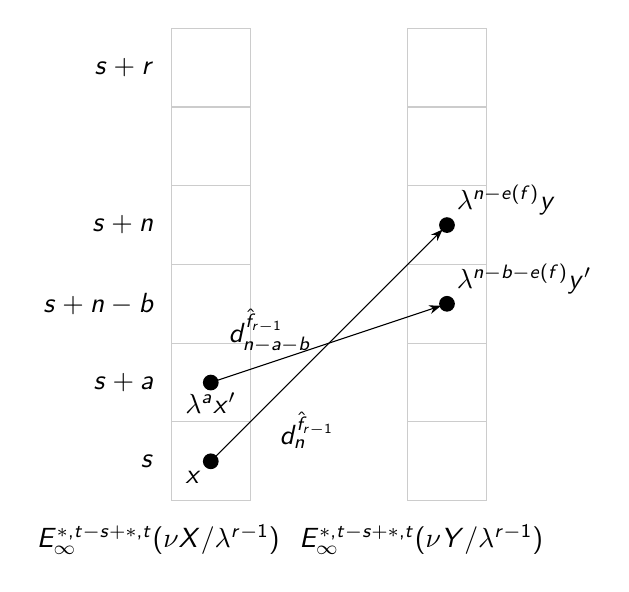
\begin{tikzpicture}
    % Draw grid
    \tikzgrid{0}{1}{0}{6}
    \tikzgrid{3}{4}{0}{6}

    % Draw bullets
    \coordinate (x) at (0, 0);
    \coordinate (x1) at (0, 1);
    \coordinate (y) at (3, 3);
    \coordinate (y1) at (3, 2);

    \fill (x) circle (0.1) node[below left] {$x$};
    \fill (y) circle (0.1) node[above right] {$\lambda^{n-e(f)} y$};
    \fill (x1) circle (0.1) node[below] {$\lambda^ax^\prime$};
    \fill (y1) circle (0.1) node[above right] {$\lambda^{n-b-e(f)} y^\prime$};

    % Draw differentials
    \drawarrow (x) -- (y) node[near start,below right] {$d^{\hat f_{r-1}}_{n}$};
    \drawarrow (x1) -- (y1) node[near start,above] {$d^{\hat f_{r-1}}_{n-a-b}$};

    \node[anchor=east] at (-0.6, 0) {$s$};
    \node[anchor=east] at (-0.6, 1) {$s+a$};
    \node[anchor=east] at (-0.6, 2) {$s+n-b$};
    \node[anchor=east] at (-0.6, 3) {$s+n$};
    \node[anchor=east] at (-0.6, 5) {$s+r$};

    \node[anchor=east] at (1, -1.0) {$E_\infty^{*,t-s+*,t}(\nu X/\lambda^{r-1})$};
    \node[anchor=west] at (1, -1.0) {$E_\infty^{*,t-s+*,t}(\nu Y/\lambda^{r-1})$};
\end{tikzpicture}
}
\caption{A crossing of an $(f,E_r)$-extension}\label{fig:66241bf6}
\end{figure}

\begin{proposition}\label{prop:cross-f-Er}
    An $(f,E_r)$-extension $d_{n}^{f,E_r}(x)=y$ (\ref{eq:b98be76a}) has a crossing if and only if the synthetic $\hat f_{r-1}$-extension $d_{n}^{\hat f_{r-1}}(x)=\lambda^{n-e(f)} y$ (\ref{eq:a020bad3}) has a crossing.
\end{proposition}

\begin{proof}
    By definition a crossing of the synthetic extension (\ref{eq:a020bad3}) has form
    \begin{equation}\label{eq:f7a7a418}
        d_{n-a-b}^{\hat f_r}(\lambda^ax')=\lambda^{n-b-e(f)}y'
    \end{equation}
    for some $x'\in Z_{r-1-a}^{s+a,t+a}(X)$ and $y'\in Z_{r-1-n+b+e(f)}^{s+n-b,t+n-b}(Y)$. Consider the following commutative diagram
    $$\xymatrix{
        \Sus^{0,e(f)}\nu X/\lambda^{r-1-a} \ar[r]^-{\hat f_{r-1-a}} \ar[d]_{\lambda^a} & \nu Y/\lambda^{r-1-a} \ar[d]^{\lambda^a}\\
        \Sus^{0,e(f)+a}\nu X/\lambda^{r-1}\ar[r]_-{\hat f_{r-1}} & \Sus^{0,a}\nu Y/\lambda^{r-1}\\
    }$$
    We see that (\ref{eq:f7a7a418}) lifts to
    \begin{equation}\label{eq:5742281}
        d_{n-a-b}^{\hat f_{r-1-a}}(x')= \lambda^{n-a-b-e(f)}y''
    \end{equation}
    for some $y''\in Z_{r-1-n+b+e(f)}^{s+n-b,t+n-b}(Y)$ such that
    $$y''\equiv y'\mod B_{1+n-b-e(f)}^{s+n-b,t+n-b}(Y)$$
    where the indeterminacy $B_{1+n-b-e(f)}^{s+n-b,t+n-b}(Y)$ is introduced by dividing $\lambda^a$.
    Therefore, the differential (\ref{eq:f7a7a418}) is essential if and only if the differential (\ref{eq:5742281}) is essential and $y''\notin B_{1+n-b-e(f)}^{s+n-b,t+n-b}(Y)$. This completes the proof.
\end{proof}

\paragraph{}
The above Definition~\ref{def:41d51149}, and Proposition~\ref{prop:cross-f-Er} can be similarly defined and stated for the case $r=\infty$.

please make the precise statement.

\paragraph{}
The above definition can be similarly defined for extensions of level $l$, such that there is a crossing of a $(f,E_r)$-extension with level $l$ iff the corresponding $\hat{f}$-extension has a crossing

please make the precise statement.

\subsection{extension at $E_r$ page and hidden extensions in $Adams$ spectral sequences}
\begin{proposition}
    Consider $f: X\to Y$, $x\in Z_\infty^{s,t}(X)$ and $y\in Z_\infty^{s+n,t+n}(Y)$.
    Then
    $$d^{f,E_\infty}_n(x)=y$$
    implies that
    $$d^{f}_n(x+B_\infty^{s,t}(X))=y+B_\infty^{s,t}(Y).$$
\end{proposition}
(The implied differential could be inessential.)

\begin{proof}
  This follows directly from inverting $\lambda$, which induces a map of spectral sequences from the $\hat f$-ESS to the $f$-ESS. The induced map on the $E_0$-pages are of the following form:
    $$\xymatrix{
    Z_\infty^{s,t}(X)/B_{1+t-w}^{s,t}(X)\ar[r]^-{d^{\hat f}_0}\ar[d]_{\lambda^{-1}} & Z_\infty^{s,t}(Y)/B_{1+t-w-e(f)}^{s,t}(Y)\ar[d]^{\lambda^{-1}}\\
    E_\infty^{s,t}(X)\ar[r]^-{d^{f}_0} & E_\infty^{s, t}(Y)
    }$$
\end{proof}
\begin{remark}
    Since the synthetic Adams $E_\infty$-page contains more information than the classical Adams $E_\infty$-page, the $(f,E_\infty)$-extensions similarly provide more information compared to the classical $f$-extensions.
\end{remark}

\begin{proposition}
    Consider $f: X\to Y$, $x\in Z_\infty^{s,t}(X)$ and $y\in Z_\infty^{s+n,t+n}(Y)$.
    Then
    $$d^{f,E_\infty, l}_n(x)=y$$
    implies that
    $$d^{f}_n(x+B_\infty^{s,t}(X))=y+B_\infty^{s,t}(Y).$$
\end{proposition}
\begin{proof}
    The same as before, since we invert $\lambda$.
\end{proof}

\end{sloppy}
\end{document}
